%%%%%%%%%%%%%%%%%%%%%%%%%%%%%%%%%%%%%%%%%%%%%%%%%%%%%%%%%%%%%%%%%%%%%%%%%%
\section{Farben}
%%%%%%%%%%%%%%%%%%%%%%%%%%%%%%%%%%%%%%%%%%%%%%%%%%%%%%%%%%%%%%%%%%%%%%%%%%
%
%%%%%%%%%%%%%%%%%%%%%%%%%%%%%%%%%%%%%%%%%%%%%%%%%%%%%%%%%%%%%%%%%%%%%%%%%%
\subsection*{Vokabeln}
%%%%%%%%%%%%%%%%%%%%%%%%%%%%%%%%%%%%%%%%%%%%%%%%%%%%%%%%%%%%%%%%%%%%%%%%%%
%
\begin{supertabular}{p{2,5cm}|ll}
%
\index{jelo}
\textbf{\dots jelo} && \textit{Adjektiv}: gelb, hellgr�n \\ % no-dictionary
\textbf{jelo} && \textit{Substantiv}: Gelb, Hellgr�n \\ % no-dictionary
 && \\ % no-dictionary
%
\index{kule}
\textbf{\dots kule} && \textit{Adjektiv}: farbenfreudig \\ % no-dictionary
\textbf{kule} && \textit{Substantiv}: Farbe, Lack \\ % no-dictionary
\textbf{kule (e \dots)} && \textit{Verb, transitiv}: f�rben, anstreichen, streichen \\ % no-dictionary
 && \\ % no-dictionary
%
\index{laso}
\textbf{\dots laso} && \textit{Adjektiv}: blau, cyan \\ % no-dictionary
\textbf{laso} && \textit{Substantiv}: Blau, Cyan \\ % no-dictionary
 && \\ % no-dictionary
%
\index{loje}
\textbf{\dots loje} && \textit{Adjektiv}: rot, r�tlich \\ % no-dictionary
\textbf{loje} && \textit{Substantiv}: Rot \\ % no-dictionary
 && \\ % no-dictionary
%
\index{pimeja}
\textbf{\dots pimeja} && \textit{Adjektiv}: schwarz, dunkel \\ % no-dictionary
\textbf{pimeja} && \textit{Substantiv}: Dunkelheit, Finsternis, Schw�rze, Schatten \\ % no-dictionary
\textbf{pimeja (e \dots)} && \textit{Verb, transitiv}: verdunkeln, schw�rzen \\ % no-dictionary
 && \\ % no-dictionary
%
\index{sitelen}
\textbf{\dots sitelen} && \textit{Adjektiv}: bildlich, figurative, bildhafte, metaphorisch \\ % no-dictionary
\textbf{\dots sitelen} && \textit{Adverb}: bildlich \\ % no-dictionary
\textbf{sitelen} && \textit{Substantiv}: Bild, Abbildung, Foto, Film, Darstellung, Gem�lde \\ % no-dictionary
\textbf{sitelen (e \dots)} && \textit{Verb, transitiv}: zeichnen, malen, schreiben \\ % no-dictionary
 && \\ % no-dictionary
%
\index{walo}
\textbf{\dots walo} && \textit{Adjektiv}: wei�, hell, bleich \\ % no-dictionary
\textbf{walo} && \textit{Substantiv}: Helligkeit, Wei�e \\ % no-dictionary
\textbf{walo (e \dots)} && \textit{Verb, transitiv}: bleichen \\ % no-dictionary
%
\end{supertabular} \\
%
%%%%%%%%%%%%%%%%%%%%%%%%%%%%%%%%%%%%%%%%%%%%%%%%%%%%%%%%%%%%%%%%%%%%%%%%%%
\newpage
%
\subsection*{Farbkombinationen}
\index{Farbe}
%
\subsubsection*{Ein Farbton}

%%%%%%%%%%%%%%%%%%%%%%%%%%%%%%%%%%%%%%%%%%%%%%%%%%%%%%%%%%%%%%%%%%%%%%%%%%
%
In \textit{toki pona} gibt es keine W�rter f�r die Farben Lila, Gr�n, Grau usw.
Man kann aber Farben aus mehreren W�rtern bilden.
Man verwendet eines dieser Substantive \textit{jelo}, \textit{laso}, \textit{loje}, \textit{pimeja} oder \textit{walo}. 
Anschlie�end verwendet man diese Adjektive \textit{jelo}, \textit{laso}, \textit{loje}, \textit{pimeja} oder \textit{walo} 

\begin{supertabular}{p{5,5cm}|ll}
laso loje li ' pona, tawa mi. && Lila ist meine Lieblingsfarbe. \\
laso jelo li ' pona, tawa mi.  && Gr�n ist meine Lieblingsfarbe.  \\
loje jelo li ' pona, tawa mi.  && Orange ist meine Lieblingsfarbe.  \\
loje walo li ' pona, tawa mi.  && Rosa ist meine Lieblingsfarbe.   \\
walo pimeja li ' pona, tawa mi. && Grau ist meine Lieblingsfarbe.  \\
\end{supertabular} 

Man kann auch Farben aus einem Substantiv und mehreren Adjektiven bilden. 
Das Ziel von \textit{toki pona} ist aber die Einfachheit.
Vermeide daher komplexe Wortzusammensetzungen.
Die Reihenfolge der Farben ist �brigens egal.

\begin{supertabular}{p{5,5cm}|ll}
laso loje  li ' pona, tawa mi. && Lila ist meine Lieblingsfarbe. \\ % no-dictionary
loje laso  li ' pona, tawa mi. && Lila ist meine Lieblingsfarbe. \\
\end{supertabular}

Farben werden in der Regel als Adjektive verwendet, weil sie Substantive beschreiben. 
Die Adjektive \textit{loje} und \textit{laso} beschreiben hier das Substantiv \textit{len}.

\begin{supertabular}{p{5,5cm}|ll}
len loje laso mi li ' pona, tawa mi. && Dieses lila T-Shirt gef�llt mir. \\
\end{supertabular}

%
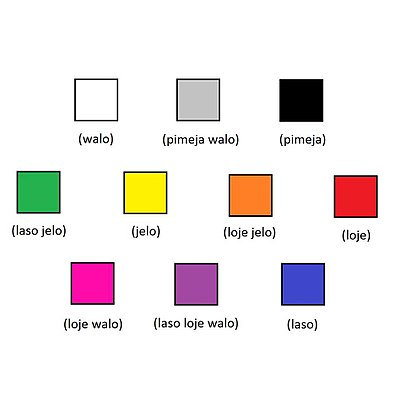
\includegraphics[scale=0.25]{colors.png}
%
%%%%%%%%%%%%%%%%%%%%%%%%%%%%%%%%%%%%%%%%%%%%%%%%%%%%%%%%%%%%%%%%%%%%%%%%%%
\subsubsection*{Muster aus mehreren Farbt�nen}
%
%%%%%%%%%%%%%%%%%%%%%%%%%%%%%%%%%%%%%%%%%%%%%%%%%%%%%%%%%%%%%%%%%%%%%%%%%%
%
Stelle dir ein rotes T-Shirt mit blauen Streifen in der Mitte vor. 
Man kann es nicht \textit{len loje laso} nennen, denn das w�rde ja ein lila T-Shirt beschreiben. 
Man muss die Farben grammatikalisch voneinander trennen. 
Jede Farbe des Musters wird mit einem Substantiv und optionalen Adjektiven beschrieben. 
Um diese Farb-Substantive mit ihren Adjektiven zu trennen verwenden wir die Konjunktion \textit{en}.
Um den gemusterten Gegenstand von seinen Farben zu trennen dient der Separator \textit{pi}.
\textit{len}, \textit{loje} und \textit{laso} sind hier Substantive. 

\begin{supertabular}{p{5,5cm}|ll}
len ni pi loje en laso li ' pona, tawa mi. && Dieses rot und blau gemusterte T-Shirt gef�llt mir. \\
tomo pi jelo en loje pi meli Susan en mije jan Ken li ' nasa, tawa mi. && Susan und Kens gelb-blau gemustertes Haus sieht seltsam aus. \\
\end{supertabular} 

%
%%%%%%%%%%%%%%%%%%%%%%%%%%%%%%%%%%%%%%%%%%%%%%%%%%%%%%%%%%%%%%%%%%%%%%%%%%
\subsection*{Das Substantiv \textit{kule}}
%
\index{\textit{kule}!Substantiv}
%%%%%%%%%%%%%%%%%%%%%%%%%%%%%%%%%%%%%%%%%%%%%%%%%%%%%%%%%%%%%%%%%%%%%%%%%%
%
Das Substantiv \textit{kule} bedeutet 'Farbe' oder 'Lack'. 

\begin{supertabular}{p{5,5cm}|ll}
ni li ' kule seme? && Was ist dies f�r eine Farbe? \\
\end{supertabular} 

%
%%%%%%%%%%%%%%%%%%%%%%%%%%%%%%%%%%%%%%%%%%%%%%%%%%%%%%%%%%%%%%%%%%%%%%%%%%
\subsection*{Das Adjektiv \textit{kule}}
%
\index{\textit{kule}!Adjektiv}
%%%%%%%%%%%%%%%%%%%%%%%%%%%%%%%%%%%%%%%%%%%%%%%%%%%%%%%%%%%%%%%%%%%%%%%%%%
%
Das Adjektiv \textit{kule} bedeutet 'farbenfreudig' oder 'bunt'. 

\begin{supertabular}{p{5,5cm}|ll}
len kule li ' pona, tawa mi. && Mir gef�llt das bunte Kleid. \\
\end{supertabular}

%
%%%%%%%%%%%%%%%%%%%%%%%%%%%%%%%%%%%%%%%%%%%%%%%%%%%%%%%%%%%%%%%%%%%%%%%%%%
\subsection*{Das transitives Verb \textit{kule}}
%
\index{\textit{kule}!Verb}
%%%%%%%%%%%%%%%%%%%%%%%%%%%%%%%%%%%%%%%%%%%%%%%%%%%%%%%%%%%%%%%%%%%%%%%%%%
%
Das transitives Verb \textit{kule} bedeutet  'f�rben'. 

\begin{supertabular}{p{5,5cm}|ll}
ona li kule ala kule e len? && F�rbt sie das Kleid? \\
mi kule e len. && Ich f�rbe das Kleid. \\
\end{supertabular} 

%
%%%%%%%%%%%%%%%%%%%%%%%%%%%%%%%%%%%%%%%%%%%%%%%%%%%%%%%%%%%%%%%%%%%%%%%%%%
\subsection*{Das Substantiv \textit{sitelen}}
%
\index{\textit{sitelen}!Substantiv}
%%%%%%%%%%%%%%%%%%%%%%%%%%%%%%%%%%%%%%%%%%%%%%%%%%%%%%%%%%%%%%%%%%%%%%%%%%
%
Das Substantiv \textit{sitelen}  bedeutet  'Bild' oder 'Gem�lde'.

\begin{supertabular}{p{5,5cm}|ll}
sitelen tawa  && Film (bewegte Bilder) \\
sitelen tawa 'Fahrenheit 9/11' li pona, tawa mi. && Ich mag den Film 'Fahrenheit 9/11'. \\
sitelen tawa 'Bowling for Columbine' li pona kin. && Der Film 'Bowling for Columbine' ist auch gut. \\
sitelen ma && Landkarte \\
o pana e sitelen ma, tawa mi. && Gib mir die Landkarte. \\
\end{supertabular} 

%
%%%%%%%%%%%%%%%%%%%%%%%%%%%%%%%%%%%%%%%%%%%%%%%%%%%%%%%%%%%%%%%%%%%%%%%%%%
\subsection*{Das Adjektiv \textit{sitelen}}
%
\index{\textit{sitelen}!Adjektiv}
%%%%%%%%%%%%%%%%%%%%%%%%%%%%%%%%%%%%%%%%%%%%%%%%%%%%%%%%%%%%%%%%%%%%%%%%%%
%
Das Adjektiv \textit{sitelen}  bedeutet  'bildlich', 'figurative', 'bildhafte', 'metaphorisch' oder '(auf)geschriebene'.

\begin{supertabular}{p{5,5cm}|ll}
toki sitelen li ' pona, tawa jan ali. && Geschriebene Sprache (Schrift) ist gut f�r alle Menschen. \\
\end{supertabular}

%
%%%%%%%%%%%%%%%%%%%%%%%%%%%%%%%%%%%%%%%%%%%%%%%%%%%%%%%%%%%%%%%%%%%%%%%%%%
%
\subsection*{Das transitives Verb \textit{sitelen}}
%
\index{\textit{sitelen}!Verb}
%%%%%%%%%%%%%%%%%%%%%%%%%%%%%%%%%%%%%%%%%%%%%%%%%%%%%%%%%%%%%%%%%%%%%%%%%%
%
Das transitives Verb \textit{sitelen} bedeutet 'malen' oder 'schreiben'.

\begin{supertabular}{p{5,5cm}|ll}
ona li sitelen ala sitelen? && Zeichnet er? \\
mi sitelen e sitelen, lon lipu. && Ich male das Bild auf Papier. \\
\end{supertabular}

%
%%%%%%%%%%%%%%%%%%%%%%%%%%%%%%%%%%%%%%%%%%%%%%%%%%%%%%%%%%%%%%%%%%%%%%%%%%
\subsection*{Das Adverb \textit{sitelen}}
%
\index{\textit{sitelen}!Adverb}
%%%%%%%%%%%%%%%%%%%%%%%%%%%%%%%%%%%%%%%%%%%%%%%%%%%%%%%%%%%%%%%%%%%%%%%%%%
%
Das Adverb \textit{sitelen}  bedeutet 'bildlich'.

\begin{supertabular}{p{5,5cm}|ll}
ona li toki sitelen e ni. && Sie sagt dies sehr bildlich. \\
\end{supertabular}

%
%%%%%%%%%%%%%%%%%%%%%%%%%%%%%%%%%%%%%%%%%%%%%%%%%%%%%%%%%%%%%%%%%%%%%%%%%%
\newpage
%
\subsection*{�bungen (Antworten siehe ~\pageref{'colors'})}
%%%%%%%%%%%%%%%%%%%%%%%%%%%%%%%%%%%%%%%%%%%%%%%%%%%%%%%%%%%%%%%%%%%%%%%%%%
%
Schreibe bitte die Antworten auf einen Zettel und �berpr�fe sie anschlie�end. 

\begin{supertabular}{p{5,5cm}|ll}
Der Slot nach der Konjunktion \textit{en} kann welche Worart(en) beinhalten? &&   \\ % no-dictionary
Wie werden Farbmuster eines Gegenstandes in \textit{toki pona} beschrieben? &&  \\ % no-dictionary
Wie werden Farbt�ne beschrieben, f�r die es kein Wort in \textit{toki pona} gibt? &&  \\ % no-dictionary
Der Slot nach dem Separator \textit{pi} kann welche Worart(en) beinhalten? &&   \\ % no-dictionary
Welche Wortarten haben die W�rter f�r Farben in \textit{toki pona}? &&  \\ % no-dictionary
\end{supertabular}

Versuche diese S�tze zu �bersetzen. 
Mit dem Tool \textit{Toki Pona Parser} (\cite{www:rowa:02}) kann man Rechtschreibung und Grammatik �berpr�fen. 

\begin{supertabular}{p{5,5cm}|ll}
Ich sehe die blaue Tasche nicht. &&   \\ % no-dictionary
Kleine gr�ne Menschen kamen vom Himmel. &&   \\ % no-dictionary
Ich mag die Farbe Lila.  &&  \\ % no-dictionary
Der Himmel ist blau. &&   \\ % no-dictionary
Siehe diesen roten K�fer.  &&  \\ % no-dictionary
Ich brauche die Landkarte.  &&  \\ % no-dictionary
Schaust du dir 'Akte-X' an? &&  \\  % no-dictionary
Welche Farbe magst du? &&  \\  % no-dictionary
Ist es rot? &&  \\ % no-dictionary
\end{supertabular}

\begin{supertabular}{p{5,5cm}|ll}
ni li pimeja ala pimeja e suno? &&  \\ % no-dictionary
suno li ' jelo. &&   \\ % no-dictionary
telo suli li ' laso.  &&  \\ % no-dictionary
mi wile moku e kili loje.  &&  \\ % no-dictionary
ona li kule e tomo tawa. &&   \\ % no-dictionary
len pi loje en laso pi meli sina li ' pona, tawa mi.  &&   \\ % no-dictionary
\end{supertabular} 

Ein kleines Gedicht.

\begin{supertabular}{p{5,5cm}|ll}
ma mi li ' pimeja. && \\ % no-dictionary
kalama ala li lon && \\ % no-dictionary
mi lape. mi sona. && \\ % no-dictionary
\end{supertabular} 
%%%%%%%%%%%%%%%%%%%%%%%%%%%%%%%%%%%%%%%%%%%%%%%%%%%%%%%%%%%%%%%%%%%%%%%%%%
% eof
